\documentclass[12pt,a4paper,twoside,openright,titlepage,final]{article}
\usepackage{fontspec}
\usepackage{amsmath}
\usepackage{amsfonts}
\usepackage{amssymb}
\usepackage{makeidx}
\usepackage{graphicx}
\usepackage[hidelinks,unicode=true]{hyperref}
\usepackage[spanish,es-nodecimaldot,es-lcroman,es-tabla,es-noshorthands]{babel}
\usepackage[left=3cm,right=2cm, bottom=4cm]{geometry}
\usepackage{natbib}
\usepackage{microtype}
\usepackage{ifdraft}
\usepackage{verbatim}
\usepackage[nottoc]{tocbibind}
\usepackage{pdflscape}
\usepackage[obeyDraft]{todonotes}
\ifdraft{
	\usepackage{draftwatermark}
	\SetWatermarkText{BORRADOR}
	\SetWatermarkScale{0.7}
	\SetWatermarkColor{red}
}{}
\usepackage{booktabs}
\usepackage{longtable}
\usepackage{calc}
\usepackage{array}
\usepackage{caption}
\usepackage{subfigure}
\usepackage{footnote}
\usepackage{url}
\usepackage[titletoc]{appendix}

\setsansfont[Ligatures=TeX]{texgyreadventor}
\setmainfont[Ligatures=TeX]{texgyrepagella}
\setmonofont{FreeMono}

\usetikzlibrary{decorations.pathreplacing}

%*******************************************************
%                 NO MODIFICAR
\newcommand*{\FSfont}[1]{%
  \fontencoding{T1}\fontfamily{#1}\selectfont}

\newlength{\tpheight}\setlength{\tpheight}{0.9\textheight}
\newlength{\txtheight}\setlength{\txtheight}{0.9\tpheight}
\newlength{\tpwidth}\setlength{\tpwidth}{0.9\textwidth}
\newlength{\txtwidth}\setlength{\txtwidth}{0.9\tpwidth}
\newlength{\drop}
%*******************************************************

% Crea una portada con los siguientes parámetros
%
% #1 : Título 
% #2 : Subtítulo
% #3 : Subsubtítulo
% #4 : Autor(es)
% #5 : Lugar
%

\newcommand*{\portada}[5]{
\begin{titlepage}
\begingroup
\vspace*{1cm}
\drop = 0.2\txtheight
\centering
\vfill
{\Huge \scshape #1}\\[\baselineskip]
{\Large \textbf{#2}}\\[\baselineskip]
{\Large \scshape #3}\\[\baselineskip]
\vspace*{0.3cm}
{\large \textit{#4}}\\[0.5\drop]

\includegraphics[scale=0.35]{./imagenes/logoURJC.jpg}
\vspace*{1.5cm}

{\large \scshape #5, \today} \par
\begin{center}
\end{center}
\vfill\null
\endgroup
\end{titlepage}
}
 %*****************************************************
 


\author{José Ignacio Escribano}

\title{}

\setlength{\parindent}{0pt}

\begin{document}

\pagenumbering{alph}
\setcounter{page}{1}

\portada{Caso Práctico III}{Minería de datos}{Estimación y predicción con máquinas de vectores soporte}{José Ignacio Escribano}{Móstoles}

\listoffigures
\thispagestyle{empty}
\newpage

\listoftables
\thispagestyle{empty}
\newpage

\tableofcontents
\thispagestyle{empty}
\newpage


\pagenumbering{arabic}
\setcounter{page}{1}

\section{Introducción}

En este caso práctico veremos cómo aplicar las máquinas de vectores soporte para predecir la densidad de una viga. Aplicaremos distintos tipos de kernel para mejorar el ajuste. Por último, calcularemos el número mínimo de densidades para conseguir que la función de ajuste siga las especificaciones marcadas por los ingenieros. 

\section{Resolución de las cuestiones de evaluación}

A continuación, resolveremos las cuestiones de evaluación planteadas.

\subsection{Cuestión 1}

Comenzando representando la función de la distancia (en pulgadas) frente a la densidad de la viga2 (Figura~\ref{fig:plot_viga2_inicial}).\\

\begin{figure}
\centering
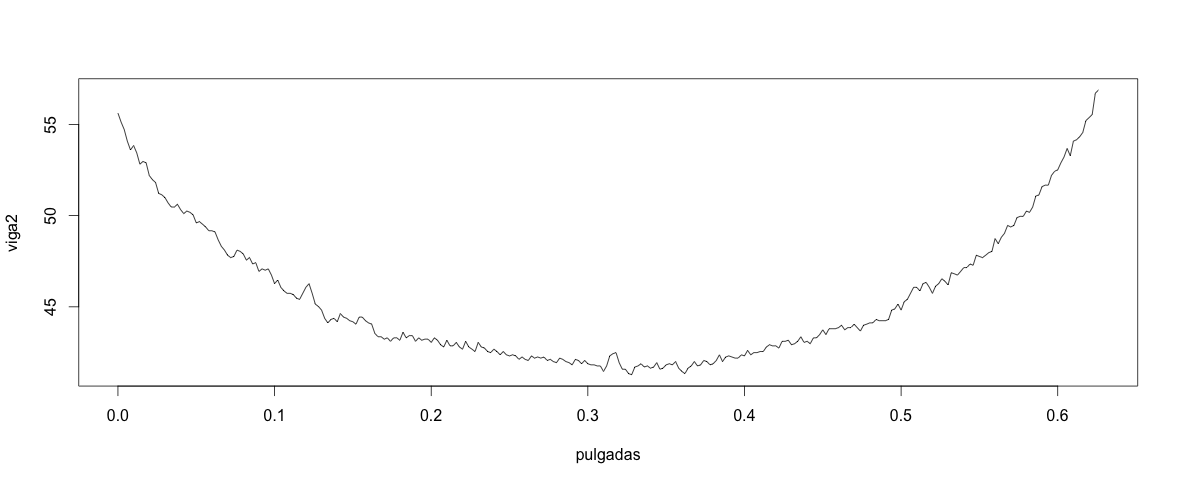
\includegraphics[width=0.8\linewidth]{imagenes/plot_viga2_inicial}
\caption{Función de la distancia frente a la densidad}
\label{fig:plot_viga2_inicial}
\end{figure}

Seleccionamos 25 puntos al azar para intentar predecir a partir de éstos los restantes. Los puntos elegidos al azar son los siguientes:

\begin{verbatim}
53.44 50.18 48.67 46.94 45.15 44.44 43.55 43.30 43.61 
42.55 42.31 42.37 42.19 42.06 41.76 41.70 41.64 42.31 
43.11 43.11 46.34 46.27 47.28 52.20 56.71
\end{verbatim}

Representamos los datos de entrenamiento en un diagrama de dispersión (Figura~\ref{fig:plot_datos_entrenamiento})\\

\begin{figure}
\centering
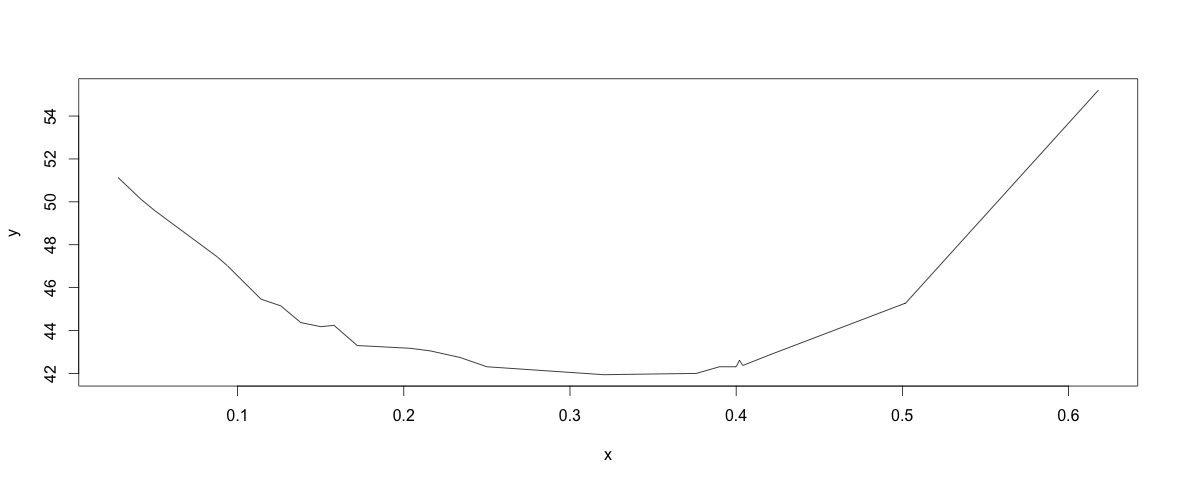
\includegraphics[width=0.8\linewidth]{imagenes/plot_datos_entrenamiento}
\caption{Función de la distancia frente a la densidad con los datos de entrenamiento}
\label{fig:plot_datos_entrenamiento}
\end{figure}

Con estos datos entrenaremos el SVM, y los restantes harán de test para comprobar la precisión del ajuste calculado.\\

Probamos el SVM con un kernel lineal y comprobamos la bondad del ajuste (Figura~\ref{fig:plot_kernel_lineal}).\\

\begin{figure}
\centering
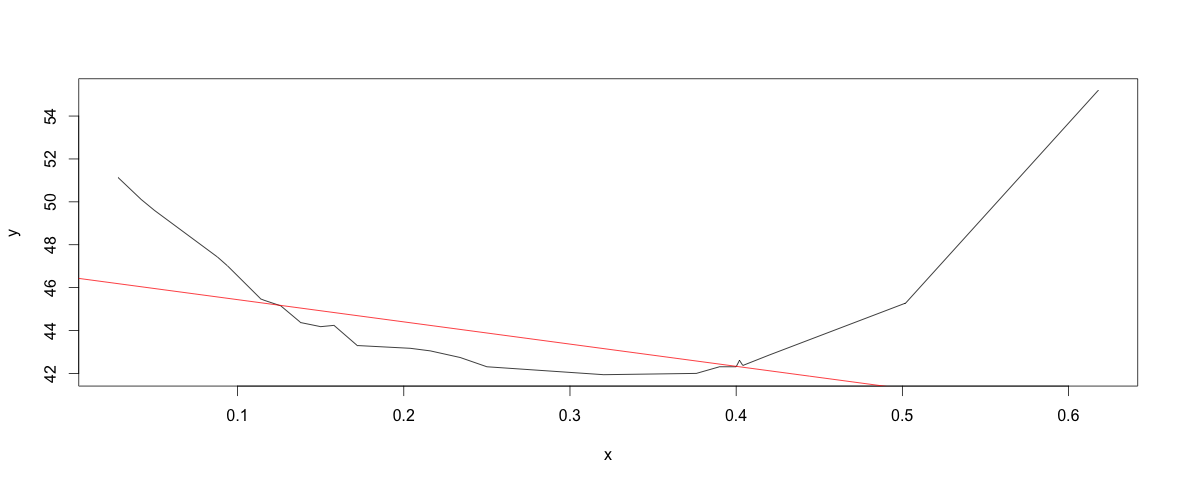
\includegraphics[width=0.8\linewidth]{imagenes/plot_kernel_lineal}
\caption{Predicción con un kernel lineal}
\label{fig:plot_kernel_lineal}
\end{figure}

Vemos que este kernel da un muy mal ajuste, por lo que probamos con un kernel no lineal con parámetros épsilon = 2, C = 100 y kernel radial con gamma = 40. La predicción de este nuevo modelo se puede ver en la Figura~\ref{fig:plot_kernel_no_lineal}.\\

\begin{figure}
\centering
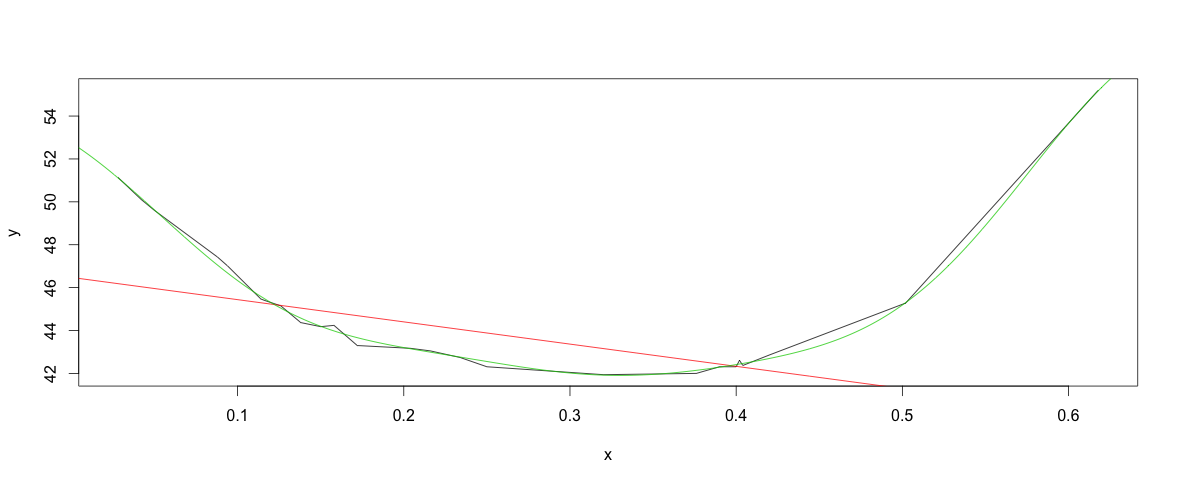
\includegraphics[width=0.8\linewidth]{imagenes/plot_kernel_no_lineal}
\caption{Predicción con un kernel no lineal}
\label{fig:plot_kernel_no_lineal}
\end{figure}

Observamos que este modelo, sí ajusta con bastante exactitud la función de la densidad.\\

Calculamos la media y la desviación típica del error del modelo. La media es 0.2701867 y la desviación típica, 0.2947849, valores muy bajos, por debajo de los valores especificados por los ingenieros.

\subsection{Cuestión 2}

De acuerdo a los datos de media y desviación típica del error, tenemos que el error se encuentra bastante por debajo de 5, el valor especificado por los ingenieros como el límite de la calidad de la viga. Por tanto, tomando sólo 25 muestras, tenemos un excelente modelo que permitirá ahorrar costes.\\

Los datos proporcionados al fabricante serán los 25 datos de entrenamientos juntos con los 289 predichos por el SVM. Ésto es, los datos de entrenamiento son:

\begin{verbatim}
53.44 50.18 48.67 46.94 45.15 44.44 43.55 43.30 43.61 
42.55 42.31 42.37 42.19 42.06 41.76 41.70 41.64 42.31 
43.11 43.11 46.34 46.27 47.28 52.20 56.71
\end{verbatim}

y los datos predichos 

\begin{verbatim}
53.28458 53.17671 53.06670 52.95461 52.84048 52.72439 52.60639 
52.48655 52.36492 52.24157 51.86188 51.73232 51.60138 51.46912 
51.33563 51.20096 51.06520 50.92842 50.79069 50.51270 50.37258 
50.23183 50.09051 49.94870 49.80649 49.66395 49.52117 49.37822 
49.23519 49.09215 48.94918 48.80638 48.66381 48.52157 48.37973 
48.23837 48.09757 47.95742 47.81800 47.54165 47.40488 47.13453 
47.00112 46.73816 46.60877 46.48087 46.35453 46.22980 46.10677 
45.98550 45.86603 45.74845 45.63280 45.51914 45.40752 45.29800 
45.19061 44.98244 44.88172 44.78331 44.68723 44.59351 44.50217 
44.41324 44.32673 44.24266 44.16104 44.08187 44.00515 43.93090 
43.85909 43.78972 43.72278 43.65825 43.59610 43.53632 43.47888 
43.42374 43.27176 43.22543 43.18119 43.13898 43.09875 43.06044 
43.02398 42.98932 42.95638 42.92510 42.89540 42.86721 42.84046
42.81507 42.79096 42.76807 42.74630 42.72558 42.70584 42.68699 
42.66895 42.65165 42.63501 42.61895 42.60340 42.58829 42.57355 
42.55911 42.54489 42.53085 42.51691 42.50302 42.48913 42.47517 
42.46112 42.44691 42.41788 42.40300 42.38783 42.37234 42.35653 
42.34037 42.32386 42.30698 42.27213 42.25418 42.23588 42.21725 
42.15964 42.13995 42.12008 42.07994 42.05976 42.03958 42.01944 
41.99939 41.97951 41.95984 41.94044 41.92138 41.90273 41.88453 
41.86687 41.84980 41.83339 41.81771 41.80281 41.77565 41.76350 
41.75239 41.74237 41.73351 41.72585 41.71944 41.71433 41.71057 
41.70820 41.70724 41.70975 41.71326 41.71831 41.72491 41.73308 
41.74283 41.75416 41.76708 41.78157 41.79764 41.83443 41.85512 
41.87730 41.90095 41.92604 41.95253 41.98038 42.00954 42.07164 
42.10448 42.13843 42.17345 42.20947 42.24645 42.28432 42.32301
42.36248 42.40267 42.48492 42.52689 42.56932 42.61219 42.65542 
42.69897 42.74279 42.78684 42.83107 42.87546 42.96453 43.00916 
43.05384 43.09853 43.14323 43.18794 43.23266 43.27738 43.32213 
43.36691 43.41176 43.45670 43.50176 43.54699 43.59243 43.63814 
43.68417 43.73059 43.77747 43.82488 43.87291 43.92163 43.97114 
44.02153 44.07290 44.12536 44.17901 44.23396 44.34820 44.40773 
44.46902 44.53220 44.59738 44.66469 44.73424 44.80617 44.88058 
44.95760 45.03734 45.11993 45.20546 45.29405 45.38581 45.48084 
45.57922 45.68106 45.78643 45.89543 46.00811 46.12455 46.24480 
46.36893 46.49697 46.62896 46.76492 46.90489 47.04886 47.19684 
47.34883 47.50480 47.66473 47.82859 47.99632 48.34320 48.52220 
48.70480 48.89090 49.08041 49.27321 49.46918 50.07474 50.28199 
50.49166 50.70360 50.91761 51.13351 51.35111 51.79060 52.01208
52.23442 52.45741 52.68083 52.90444 53.12802 53.35134 53.57415 
53.79622 54.01732 54.23721 54.45565 54.67240 54.88723 55.09990 
55.31018 55.51784
\end{verbatim}

La Figura~\ref{fig:plot_fabricante} muestra estos datos en forma de gráfica.\\

\begin{figure}
\centering
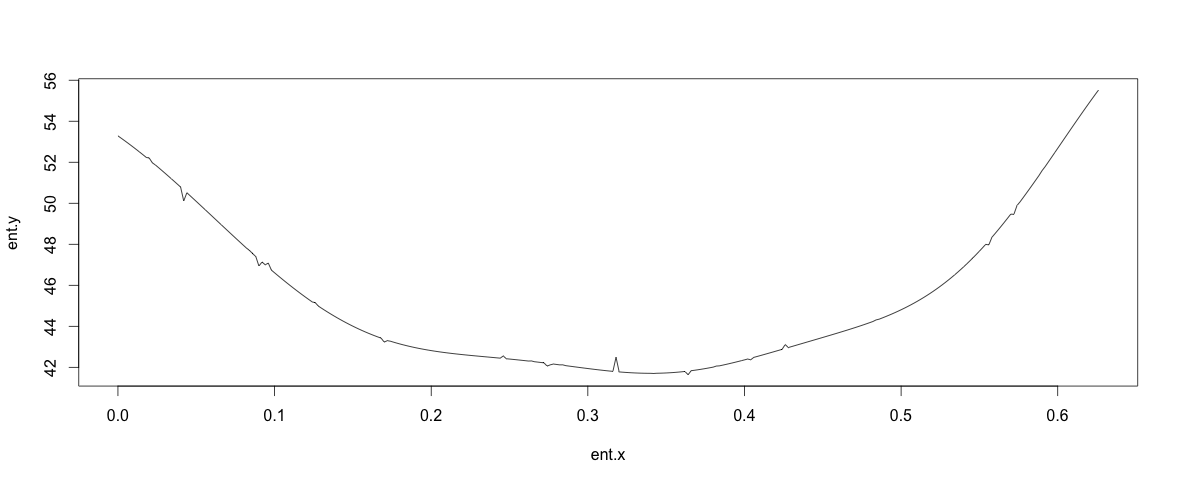
\includegraphics[width=0.8\linewidth]{imagenes/plot_fabricante}
\caption{Datos proporcionados al fabricante}
\label{fig:plot_fabricante}
\end{figure}

\subsection{Cuestión 3}

Para obtener el número mínimo de densidades para que el modelo siendo válido, es decir, el error absoluto en las predicciones sea mínimo, tomamos una muestra de 2 densidades aleatoriamente, entrenamos el modelo, y lo verificamos con los datos restantes. Si se cumple que el error absoluto es menor que 5, nos quedamos con él, en caso contrario aumentamos en una unidad el número de densidades.\\

Implementando el algoritmo anterior en R, tenemos que este número mínimo de densidades es 2. En la Figura~\ref{fig:2sv} se puede ver la función predicha por este SVM junto a la función original.\\

\begin{figure}
\centering
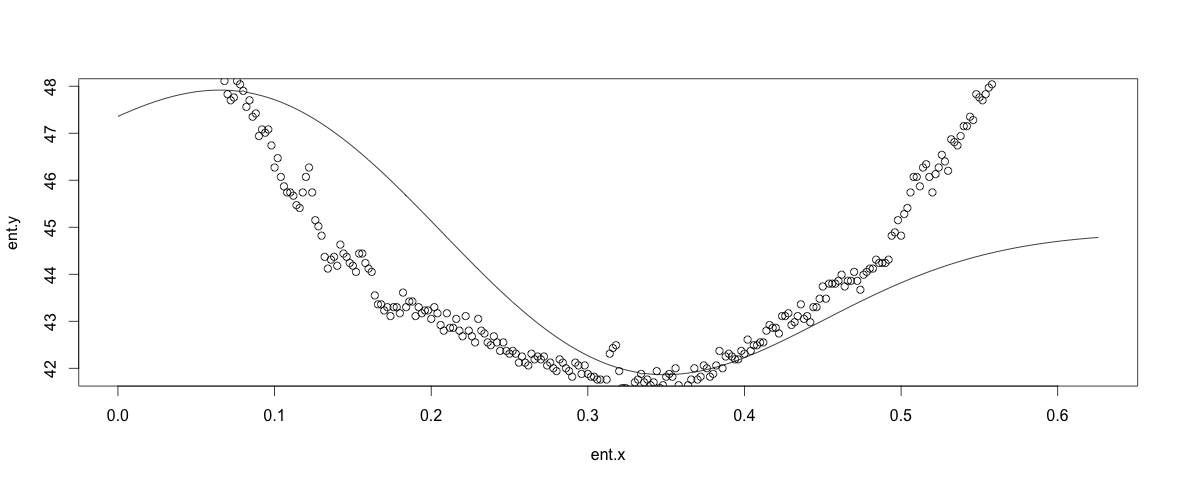
\includegraphics[width=0.8\linewidth]{imagenes/2sv}
\caption{Función predicha por con dos vectores soporte}
\label{fig:2sv}
\end{figure}

Vemos que en algunos lugares el ajuste es bastante bueno, mientras que en otros es bastante malo, aunque el ajuste cumple con las especificaciones fijadas por los ingenieros (Tabla~\ref{tbl:medias}), aunque tiene una desviación típica del error muy alta.\\

\begin{table}[htbp!]
\centering
\caption{Media y desviación típica del error absoluto según el número de densidades}
\label{tbl:medias}
\begin{tabular}{@{}ccc@{}}
\toprule
Número de densidades & Media     & Desviación típica \\ \midrule
2                    & 1.851380  & 2.507192          \\
3                    & 1.957093  & 2.747603          \\
4                    & 2.324786  & 3.189393          \\
5                    & 1.077422  & 2.006100          \\
6                    & 1.008247  & 1.986431          \\
7                    & 1.097909  & 1.799587          \\
8                    & 0.877396  & 1.361815          \\
9                    & 0.363463  & 0.341001         \\ \bottomrule
\end{tabular}
\end{table}

Según vamos aumentando el número de vectores soportes, se va mejorando el ajuste de la función (Figura~\ref{fig:sv}).\\

\begin{figure}[htbp]
\centering
\subfigure[2 vectores soporte]{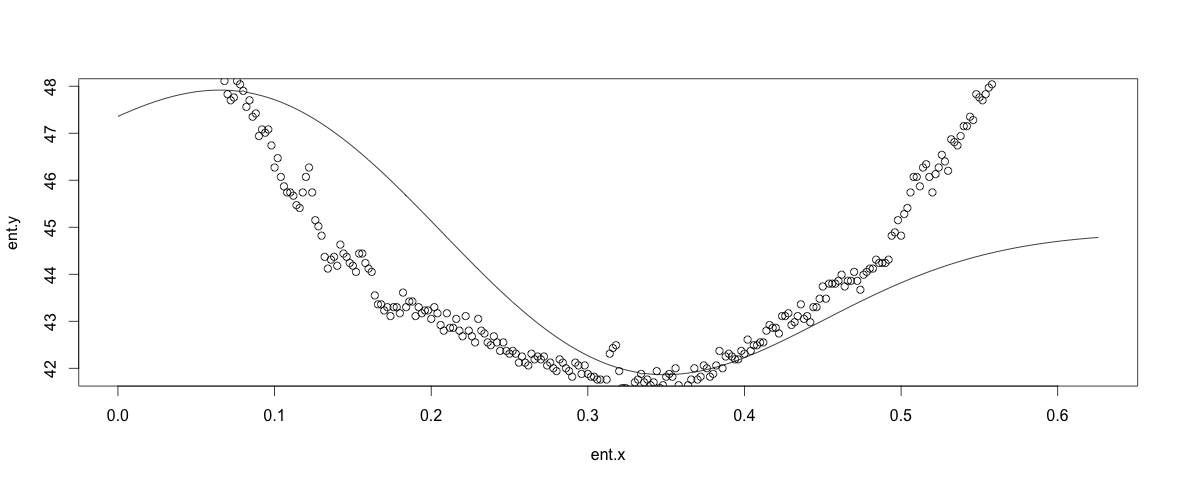
\includegraphics[width=0.45\linewidth]{imagenes/2sv}}
\subfigure[3 vectores soporte]{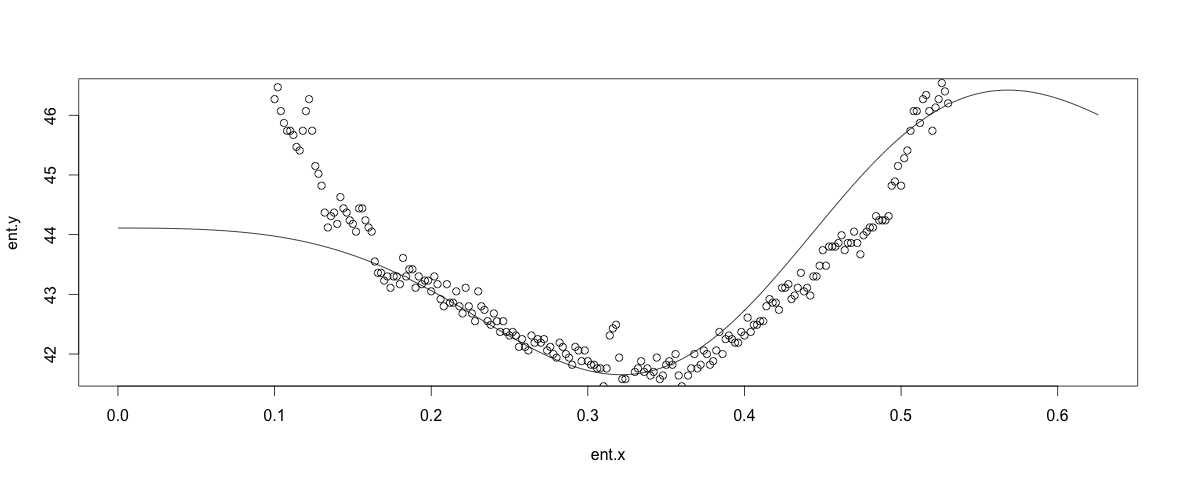
\includegraphics[width=0.45\linewidth]{imagenes/3sv}}
\subfigure[4 vectores soporte]{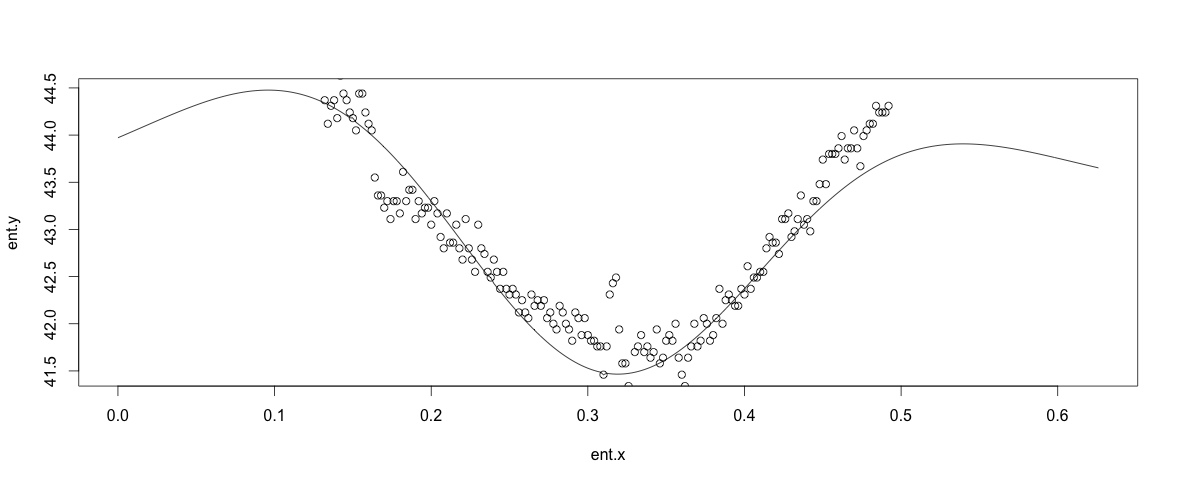
\includegraphics[width=0.45\linewidth]{imagenes/4sv}}
\subfigure[5 vectores soporte]{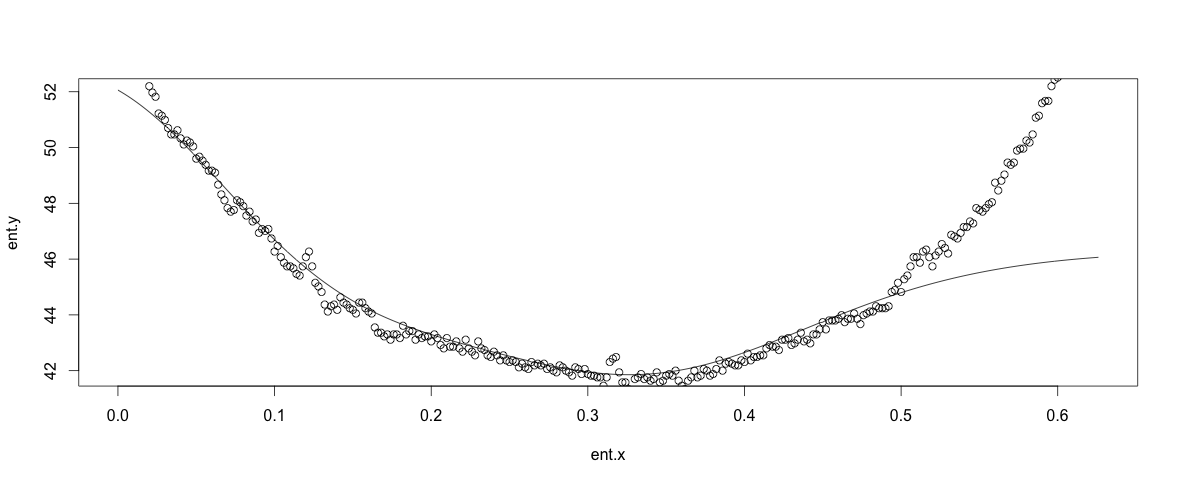
\includegraphics[width=0.45\linewidth]{imagenes/5sv}}
\subfigure[6 vectores soporte]{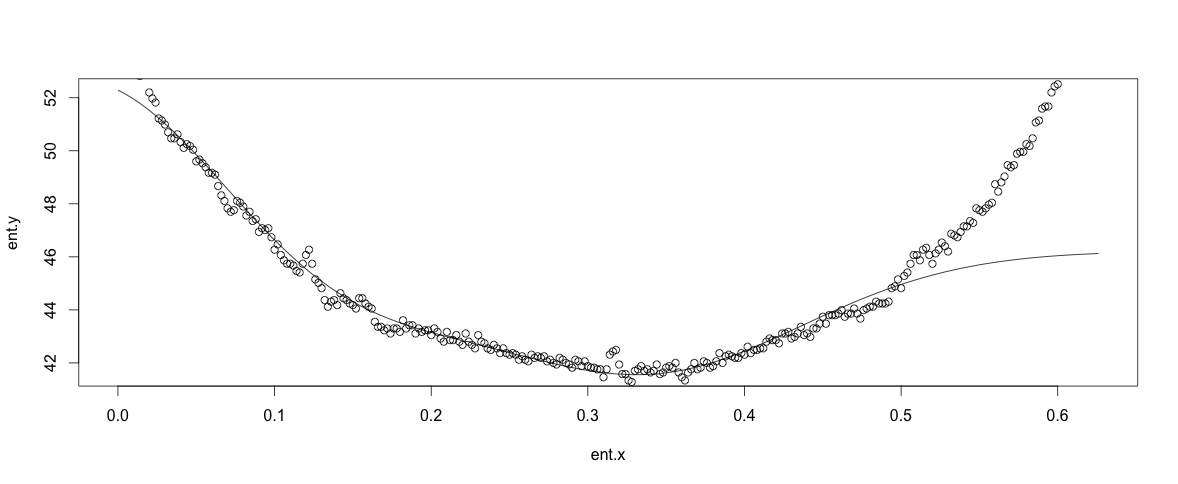
\includegraphics[width=0.45\linewidth]{imagenes/6sv}}
\subfigure[7 vectores soporte]{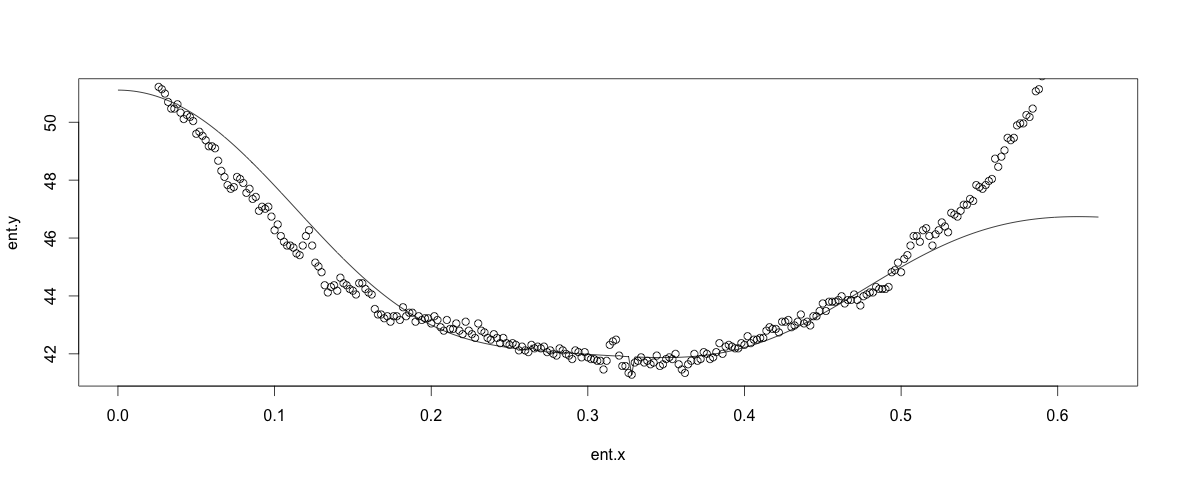
\includegraphics[width=0.45\linewidth]{imagenes/7sv}}
\subfigure[8 vectores soporte]{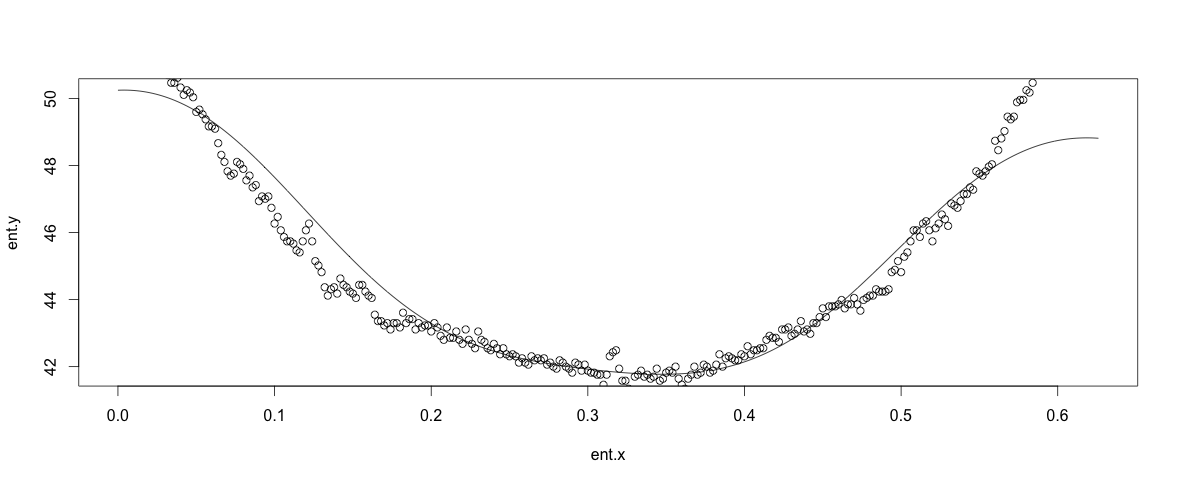
\includegraphics[width=0.45\linewidth]{imagenes/8sv}}
\subfigure[9 vectores soporte]{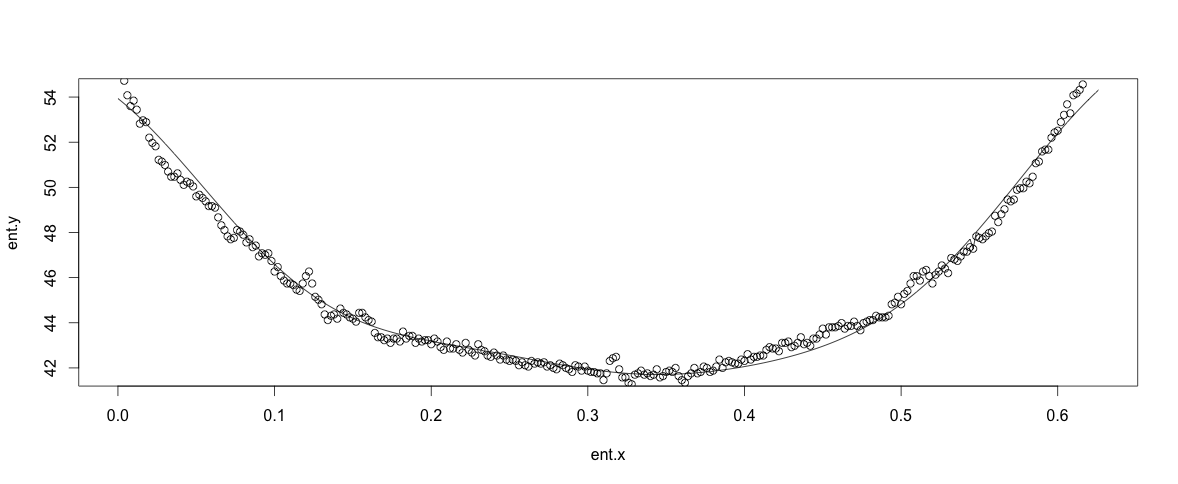
\includegraphics[width=0.45\linewidth]{imagenes/9sv}}
\caption{Función predicha por con distintos número de vectores soporte} 
\label{fig:sv}
\end{figure}

A tenor de la Tabla~\ref{tbl:medias} y la Figura~\ref{fig:sv}, todos los SVM entre 2 y 9 vectores soporte cumplen con las especificaciones de los ingenieros, aunque algunos debidos a la variabilidad de los errores no parecen óptimos.\\

En el caso de 9 vectores soporte, se observa un acusado descenso del promedio y de la desviación típica del error, por lo que parece un número de densidades asequible para ser utilizado, con su reducción de coste asociado, aunque se pueden elegir cualquiera de los demás modelos desde 2 hasta 8 vectores soporte ya que cumplen todos con las especificaciones de los ingenieros.

\section{Conclusiones}

En este caso práctico, hemos puesto en práctica lo aprendido sobre máquinas de vectores soporte, aplicándolo a una aplicación real como puede ser la predicción de la densidad de una viga. También, hemos visto cómo mejorar la predicción de una función, usando el ``kernel trick''.\\

El software científico R nos ha ayudado mucho debido a las librerías que implementan los SVM, incluyendo distintos tipos de kernel, que nos han ahorrado mucho tiempo gracias a su potencia de cálculo. 

\clearpage

\section{Código R utilizado}

\verbatiminput{caso_3.R}

\end{document}